\documentclass[11pt, a4paper, oneside, parskip=full-]{scrartcl}

% -- PREABLE

% global settings
\renewcommand\labelitemi{-}

% packages
\usepackage[utf8]{inputenc}
\usepackage{graphicx} % to embed figures
\usepackage{float} % use [H] to place fig exactly where specified in code
\usepackage{tabularx} % table with columns that fill width of page using X
\usepackage{booktabs} % table utilities like \midrule
\usepackage{multirow} % span multiple rows in table
\usepackage{enumitem} % pass key-value config to itemize and enumberable
\usepackage{hyperref} % for links and urls
\usepackage[style=numeric,backend=biber,sorting=none]{biblatex} % For citing
\usepackage{listings} % For code snippets

\addbibresource{thesis.bib}

\graphicspath{ {img/} } % path where grahics are stored

% title page parameters
\title{Open-Source Tools Sandbox \& Data Stories - New tools for GIS workshops}
\author{Marc Folini}
\date{May 2022}

% -- BODY
\begin{document}

%-------------
% TITLE, ABSTRACT
%-------------
\begin{titlepage}
  \pagenumbering{Roman}
  \setcounter{page}{1}
  % create title page
  \clearpage\maketitle
  \thispagestyle{empty}
  % abstract
  \begin{abstract}
    It is desirable in GIS workshops to supplement the theoretical concepts with
    hands-on exercises in order for participants to become an active part in the
    learning experience. This requires that participants have access to an
    environment that provides the necessary software and data - ideally with
    minimal setup effort, independent of the system they use and easy to
    uninstall without leaving traces after the workshop. Different approaches
    were evaluated, and container technology was found to be a good fit to
    abstract away the hassle of setting up the tools and infrastructure. A proof
    of concept of what will be referred to as \emph{Sandbox environment} was
    implemented and published as open source project.

    Furthermore, this thesis explored the concept of \emph{data stories}. A data
    story provides selected raw data, a motivating tangible goal and
    instructions that connect the raw data to the goal. It allows participants
    to fully focus on how the different tools interact with the data itself and
    other tools to achieve a meaningful result. This is in contrast to the
    majority of tutorials, which are tool focused and to which data is secondary
    to teach the necessary functionalities of a specific tool. An example data
    story was implemented whereby open data from the city of Zürich is used to
    derive a map showing what percentage of roads in each district are suitable
    for biking. Participants learn about the GDAL\cite{gdal} command line tools
    to inspect datasets and load them into PostGIS\cite{postgis}, where spatial
    processing and aggregation is performed. The result is made available as a
    new dataset to be consumed and styled in QGIS\cite{qgis}.
  \end{abstract}
\end{titlepage}

%-------------
% TABLE OF CONTENT
%-------------
\newpage
\tableofcontents

%-------------
% INTRODUCTION
%-------------
\newpage
\pagenumbering{arabic}
\setcounter{page}{1}
\section{Introduction}
Educational GIS\footnote{Geographic Information System (GIS).} workshops face a
few particular challenges, two of which are central to this thesis. Firstly, it
is desirable for participants to experience theoretical concepts hands-on for
themselves. The challenge here lies in providing all participants with access to
the respective software and data with minimal setup efforts. Secondly, the GIS
landscape today consists of many components covering the whole data lifecycle
from initial data exploration to visualization and distribution. Together with
the myriad of commercial and open source tools for each component, this might be
overwhelming to people new to the field.

This thesis was written as part of the CAS RIS 2021/22\footnote{Certificate of
advanced studies (CAS) in GIS (in German RIS) offered by ETH Zurich.}. It
explores the two above-mentioned challenges in the context of the CAS and aims
to address them on two different levels:
\begin{enumerate}
  \item \textbf{Infrastructure} In order to provide participants access to a
  variety of software with minimal setup effort the concept of a \emph{Sandbox
  environment} is explored. The requirements and components to be implemented in
  a first version were chosen to support the content of this thesis' further
  education curriculum.
  \item \textbf{Content} In order to help participants to make sense of the
  Sandbox components and their interactions, the concept of a \emph{data story}
  was explored. Each data story has a tangible data driven use case and then
  provides guidance on how available technologies and tools interact with the
  data to achieve the desired result.
\end{enumerate}


%-------------
% REQUIREMENTS
%-------------
\section{Requirement analysis} \label{sectionrequirements}

The content of the CAS RIS was analyzed for potential hands-on exercises. From
these findings functional and non-functional requirements\footnote{Functional
requirements specify the tasks an application must be able to perform.
Non-functional requirements specify additional aspects about the application
performing the task, for example usability, look and feel or performance. } for
a Sandbox were then derived.

% Content analyis
%-------------
\subsection{Content analysis}
At the time of writing the CAS course consisted of four weeks of content modules
on a wide variety of topics. Each module was screened with a focus on where a
Sandbox could facilitate hands-on experiences without substantially altering the
module structure or material. Modules focusing primarily on usage of proprietary
software like ArcGIS were ignored. Table \ref{tab:tContentAnalysis} shows the
results of the analysis.

\begin{table}[!htbp]
  \centering
  \caption{Content analysis of existing lectures for Sandbox facilitation potential.}
  \label{tab:tContentAnalysis}
  \begin{tabularx}{\textwidth}{lX}
    \toprule
    % header row start
    \textbf{Module} & \textbf{Sandbox facilitation potential} \\
    \midrule
    % row start
    Interoperabilität &
      \begin{itemize}[left=0pt,nosep,before={\begin{minipage}[t]{\hsize}},after
      ={\end{minipage}}]
      \item Inspection of and conversion between various data formats.
      \item Read Shapefile into a spatial database.
      \end{itemize}\nointerlineskip\\
    \midrule
    % row start
    SQL & Write and run basic SQL queries on sample data. \\
    \midrule
    % row start
    Geodatenbanken &
    \begin{itemize}[left=0pt,nosep,before={\begin{minipage}[t]{\hsize}},after
    ={\end{minipage}}]
      \item Run basic spatial queries on sample data.
      \item Perform spatial aggregation on sample data.
      \end{itemize}\nointerlineskip\\
    \midrule
    % multirow(4) start
    Geometrische Methoden & \multirow[t]{4}{*}{Run simple examples on sample
    data.} \\
    \cmidrule(r){1-1} Topologische Methoden &  \\
    \cmidrule(r){1-1} Mengenmethoden &  \\
    \cmidrule(r){1-1} Statistische Methoden &  \\
    \midrule
    % row start
    Einführung in Python & Self-study introduction of python basics. \\
    \midrule
    % row start
    Internet und GIS I \& II &
      \begin{itemize}[left=0pt,nosep,before={\begin{minipage}[t]{\hsize}},after
      ={\end{minipage}}]
      \item Load data from OGC web services WMS/WFS/WCS\footnote{The Open
      Geospatial Consortium (OGC) is a worldwide community to improve the access
      to geospatial data by various means such as developing standards. Such
      standards for the web include Web Map Service (WMS), Web Feature Service
      (WFS) and Web Coverage Service (WCS) to load styled map images, simple
      geometry features and raster data via HTTP respectively.}.
      \item Optional: Consume WMS with QGIS. \end{itemize}\nointerlineskip \\
    \midrule
    % row start
    Projekt Internet \& GIS &
      \begin{itemize}[left=0pt,nosep,before={\begin{minipage}[t]{\hsize}},after
      ={\end{minipage}}]
      \item Use geodatabase as data source for OGC server.
      \item Create style and serve data as WMS.
      \item Consume WMS with QGIS. \end{itemize}\nointerlineskip \\
    \bottomrule
  \end{tabularx}%
\end{table}%

% Functional requirements
%-------------
\subsection{Functional requirements}
The following functional requirements were identified for the Sandbox to be
useful in realizing the potential identified in the content analysis:
\begin{itemize}
  \item A spatial database is available together with utilities to import and
  query data.
  \item An OGC server implementation is available. There is a way to read
  predefined example data, read data from the user's system or connect to the
  Sandbox spatial database.
  \item An OGC client implementation is available, which can interact with the
  Sandbox OGC server or any other OGC service publicly available on the
  internet.
  \item The GDAL command line utilities, particularly gdalinfo and ogr2ogr, are
  available. There is a way to read either predefined example data or read data
  from the user's system.
  \item An environment to write and run python scripts which make use of the
  python geo-ecosystem. A use case would be to provide illustrative examples for
  the concepts of geometry, topology and spatial statistics.
\end{itemize}

% Non-Functional requirements
%-------------
\subsection{Non-Functional requirements}
\begin{itemize}
  \item Users can create content which is persisted between usages of the
  Sandbox.
  \item There is a possibility to ship example scripts and data as part of the
  Sandbox.
  \item Creation and distribution of data stories that are compatible with the
  tools of the Sandbox should be possible without in-depth technological
  knowledge.
  \item The Sandbox can be installed effortlessly and in a uniform way across
  the most common operating systems, namely Apple OS, Linux and Windows.
  \item The Sandbox can be uninstalled without leaving traces on the operating
  system.
  \item Turning the Sandbox on/off and accessing components should not require
  any programming knowledge.
  \item A partial or total reset of applications and data is possible in case
  something got messed up.
  \item Usage is not coupled to the duration of the CAS course or otherwise
  restricted (e.g. via externally controlled credentials).
\end{itemize}

%-------------
% SANDBOX
%-------------
\section{Sandbox}

% Existing projects
%-------------
\subsection{Existing projects}
Google search engine was used to look for already existing similar projects
using various combinations of the terms \emph{gis}, \emph{geo}, \emph{Sandbox},
\emph{workshop}, \emph{playground} and \emph{spatial}. No project was found that
satisfied the requirements outlined in section \ref{sectionrequirements}, but
some noteworthy findings are listed below.

\begin{itemize}
  \item Joeyklee's Geosandbox\cite{project-joeyklee} is a collection of
  tutorials which seems to focus on JavaScript client side mapping libraries
  such as Leaflet. It is not suitable for our purpose but mentioned here for the
  very similar name Geosandbox to avoid confusion.
  \item IDRE Sandbox\cite{project-idre} does not provide any easy access to
  tools, but seems to be a collection of workshops and tutorials. It is
  mentioned here because the interesting goals and presentation of some
  workshops served as inspiration for the data story of this thesis.
  \item Digital Earth Australia (DEA) Sandbox\cite{project-dea} was a wonderful
  discovery. After creating a free account a cloud hosted
  JupyterLab\cite{jupyterlab} platform with extensive python Jupyter Notebooks
  provide an interactive engaging experience to learn about the analysis of
  satellite imagery and much more. The DEA Sandbox was a major inspiration for
  the heavy focus use of JupyterLab in our Sandbox.
  \item Geopython Workshop Repository\cite{project-geopython} is an extensive
  knowledge hub about a broad range of geospatial topics. The workshop is built
  on python Jupyter Notebooks using a containerized JupyterLab environment with
  pre-installed libraries. Docker Compose\cite{dockercompose} is used as
  container orchestration technology. Even though the setup is too limited for
  the use case of this thesis (a spatial database is missing for example) the
  idea of using container technology to abstract away dependency management
  provided major inspiration for this thesis.
\end{itemize}

% Technology evaluation
%-------------
\subsection{Technology evaluation}

\subsubsection{High level architectural approaches}
The research on existing projects and further exploration of potential
technologies led to three distinct groups of architectural approaches to be
evaluated: Sandbox as direct installation on user system, Sandbox as local
containerized application and Sandbox as cloud service.

\subsubsection*{Sandbox as direct installation on user system}
It was found that only four established open-source projects (QGIS, PostGIS,
pgAdmin\cite{pgadmin} and GeoServer\cite{geoserver}) would be enough to satisfy
the major part of the functional requirements. While the roles of PostGIS as
spatial database and GeoServer as OGC data server are well-defined, the QGIS
installation is particularly interesting because it comes bundled with versions
of GDAL and python that work together well. The community has produced
installers for all major operating systems, which makes the installation
relatively straight-forward.

When it comes to non-functional requirements this approach falls short. A major
shortcoming is the lengthy and intrusive setup stemming from the lack of
separation of the Sandbox software from the rest of the user's system. Depending
on already existing software and specific configurations this approach is at
best error-prone and at worst capable to permanently alter the user's system.
Because with this approach only the tools themselves are installed, tutorials
and data stories would need to be provided in a separate way. On the positive
side, the installed tools could be used beyond the duration of the CAS course
without problems and the decoupling of the distribution of tutorials and data
stories make it easy to be updated without technical knowledge.

\subsubsection*{Sandbox as local containerized application}
Container technology has been around for decades but took off in 2013 with the
release of Docker, which provided the tools that made container technology
accessible to the broader mass. Containers allow for bundling different software
components together in a reproducible way (an image) which can be distributed
and run in an isolated manner from the rest of the hosting computer's system
(called host). Compared to virtual machines containers are very lightweight and
can be started and stopped within seconds.

This approach takes the direct installation approach one step further by running
a spatial database or an OGC data server in containers isolated from the host
system. A difference from the direct installation approach is that QGIS was
found to be not suitable as containerized application in the context of the
Sandbox because of extra configuration required on the host system for graphical
output. On a positive note, complex installation procedures can be fully
abstracted away from the user in a containerized setup as part of the image
creation process, which would allow for example to set up a JupyterLab
environment with system dependencies like GDAL in order to have access to a wide
variety of python packages from python's geo-ecosystem and GDAL terminal
commands.

The setup complexity is comparatively low, because the only prerequisite is the
installation of Docker, which is an easy and mature process for all major
operating systems at this point thanks to its huge popularity. Once installed,
the containers can be started and stopped with single commands in seconds.
Containers can also contain data which optionally can be persisted on the host
on virtual volumes. Example scripts and data stories can be distributed as part
of the container and by using volumes they can be persisted across Sandbox
restarts or selectively reset. Except for the initial installation this approach
satisfies all requirements.

\subsubsection*{Sandbox as cloud service}
The advances of container technology went hand in hand with the maturation of
the publicly available cloud. It's possible today even for a layman to run
containerized applications in the cloud at scale using a variety of managed
services ranging from authentication to load balancing.

This approach takes the local containerized approach one step further into the
cloud. Instead of bothering with the installation of Docker on the user's
computer and running the containers locally the Sandbox is made available as a
service with a simple web interface and optionally some kind of login. Some
functional requirements such as the availability of a spatial database could
even be satisfied with cloud native components such as fully managed database
services.

The advantage of a cloud service is the low entry barrier because there is no
installation required. Example data and data stories can be made readily
available as part of the container setup and resetting is as simple as starting
a new Sandbox cloud instance. This convenience comes at the price of a cost and
complexity overhead at the cloud side, because for persisting data across
sessions some form of authentication must be in place and every cloud session
uses resources which are billed by the second. Assuming the cloud Sandbox is
publicly available to fulfill the requirement that the Sandbox' usage should not
be coupled to the duration of the CAS course, further complexity arises from
implementing and maintaining security best practices against malicious attacks.
Data management is another topic which can prove challenging when it comes to
cloud services in the geospatial domain, because data usually needs to be
uploaded before being accessible and spatial data can quickly become rather
large for standard internet connection upload speeds leading to disruptions and
waiting times.

\subsubsection*{Conclusion: Sandbox as local containerized application}
All three approaches satisfy the functional requirements, so the non-functional
requirements will be used to argue for the final decision. The direct
installation approach falls short here. The local containerization approach has
some minor shortcomings when it comes to the initial installation, but shines in
almost all other areas. The cloud service approach is the opposite, shining with
a zero-effort setup but falling behind the local containerization approach in
terms of maintainability, cost, and data management.

The approach \emph{Sandbox as local containerized application} was eventually
chosen for the further implementation, because simplicity of a local setup
combined with the advantages of container technologies was found to outweigh the
cost of the initial setup, which is still orders of magnitude simpler than with
the direct installation approach.

\subsubsection{Technology evaluation for local containerized application}
The technology to be used for local containerized application has to be able to
run multiple containers which can communicate among each other as well as with
the host system and store data which is persisted beyond the lifecycle of each
container. Among many possibilities, three technologies were considered more
closely due to their popularity and the availability of detailed documentation:
Docker Compose, Docker Swarm and Minikube.

\begin{itemize}
  \item \textbf{Docker Compose} allows running multi-container applications on a
  single host. A single compose file acts as configuration for container
  lifecycle and environment as well as the networking and storage layers.
  \item \textbf{Docker Swarm}\cite{dockerswarm} shares many concepts with Docker
  Compose and can be considered an evolution towards orchestrating multiple
  containers across multiple host machines. It is also possible to run Docker
  Swarm on a single host machine.
  \item \textbf{Minikube}\cite{minikube} is a tool that lets you run a local
  version of a Kubernetes Cluster. Kubernetes is one of the most popular
  container orchestration software and at a high level similar to Docker Swarm.
  It provides its own approach towards managing containers, networking and
  storage which is generally more targeted towards large-scale enterprise
  applications.
\end{itemize}

All three technologies were evaluated on a two container setup of a spatial
database (PostGIS) and an associated administrator application (pgAdmin). While
all three technologies provided extensive documentation that allowed for
successful testing, Docker Compose proved to be the simplest solution in terms
of initial setup and ease of use, due to its single configuration file and the
targeted use case to run on a single host. To that end \emph{Docker Compose} was
chosen as the technology to implement the \emph{Sandbox as local containerized
application}.


% Architecture
%-------------
\subsection{Architecture}
The Sandbox was designed as a modular multi-container setup to be run locally by
Docker Compose. The architecture is outlined in Figure \ref{fig:sandboxsetup}.

\begin{figure}[H]
  \centering
  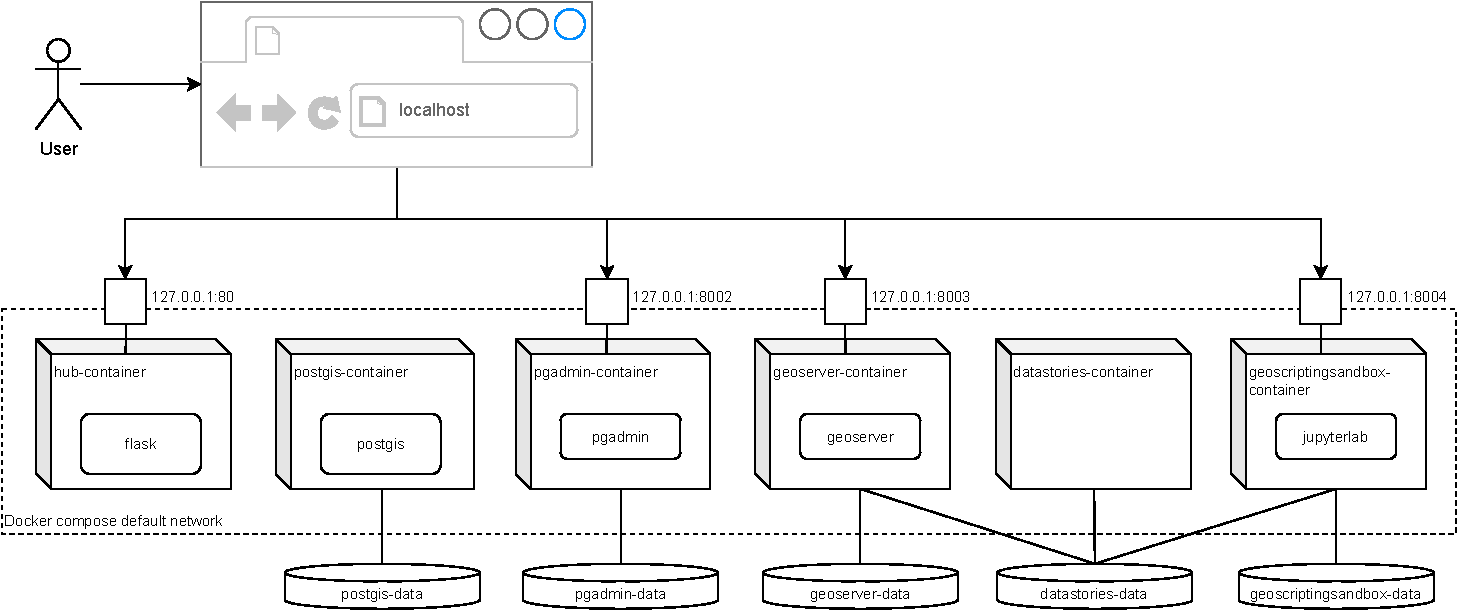
\includegraphics[width=1\textwidth]{composeSetup}
  \caption{Sandbox architecture}
  \label{fig:sandboxsetup}
\end{figure}

\subsubsection*{Containers}
At its heart the Sandbox consists of six containers, each with a distinct
purpose:

\begin{itemize}
  \item \textbf{hub-container} runs a simple web application that serves as an
  entry point and central hub for the Sandbox. Here a user finds links to access
  other Sandbox components and the relevant connection information. The hub is
  the first thing a user sees when typing \emph{localhost} in the browser after
  starting the Sandbox.
  \item \textbf{postgis-container} is a containerized version of PostGIS, a
  spatial database.
  \item \textbf{pgadmin-container} is a containerized version of pgAdmin4, a
  graphical user interface to facilitate the administration of PostgreSQL based
  databases, such as PostGIS.
  \item \textbf{geoserver-container} is a containerized version of GeoServer,
  which is an OGC data server and a reference implementation of the OGC web
  services.
  \item \textbf{geoscriptingsandbox-container} is a containerized version of
  JupyterLab, a web-based interactive development environment for python scripts
  and more. It should come bundled with various pre-installed python packages
  from the geo-ecosystem and fundamental libraries such as GDAL and
  GEOS\cite{geos}. This setup allows users to explore the python geo-ecosystem
  as well as the various command line utilities that GDAL offers. The expressive
  nature of Jupyter Notebooks is also used to visualize the data stories.
  \item \textbf{datastories-container} is called a data container because it
  serves solely as a data storage without application. It contains the data
  story related narrative in form of Jupyter Notebooks as well as the sample
  data.
\end{itemize}

\subsubsection*{Usage of volumes for persistent data storage}
Some containers make use of virtual volumes as shown in Figure
\ref{fig:sandboxsetup} to persist data across restarts of the Sandbox. Examples
include the data stored in PostGIS, the database connections set up in pgAdmin
or the data and configuration files used by GeoServer.

A special case is datastories-container, which upon each start copies all its
content to a volume datastories-data which can be accessed by other containers
such as geoscriptingsandbox-container to access the data story Jupyter
Notebooks. This pattern assures that the data stories on the volume always
correspond to the data stories container content.

\subsubsection*{Networking}
All containers are part of a virtual network managed by Docker Compose which is
isolated from the host system. In this network every container can connect to
every other container by its container name and the port exposed by the
container's application. As shown in Figure \ref{fig:sandboxsetup} some
containers also expose selected ports to the host network, which allows
interacting with the application within the container from outside the Docker
Compose network through the host network's localhost interface. This has
consequences for the user experience, because the way to connect to a certain
Sandbox component differs based on whether the connection happens from another
Sandbox component (e.g. Sandbox pgAdmin to Sandbox PostGIS) or from outside the
Sandbox (e.g. QGIS to Sandbox PostGIS) because each case uses a different
network. Hours were spent researching how to homogenize the user experience
without success and in the current implementation the Sandbox hub's connection
information makes it as explicit as possible which connection information to use
in which case.

\subsubsection*{Access to host file system}
Even though not indicated in Figure \ref{fig:sandboxsetup}, it is also possible
to grant containers access to the file system of the host machine. This seems to
contradict the basic idea of isolation but proves to be useful in certain cases.
The current Sandbox implementation creates such a link to the host file system
for the geoscriptingsandbox-container and geoserver-container with the intent to
make it easy for users to let these components make use of data saved on their
local machine.

% Implementation
%-------------
\subsection{Implementation}

This section covers the implementation of the Sandbox using Docker Compose. The
resulting implementation is provided in this thesis'
repository\cite{osgeostacksandbox} and is free to use under MIT license.

At the heart of a Docker Compose application is a configuration file, called
\emph{compose file} which describes the components of the multi-container setup
and how they interact. Each component is called a \emph{service}, which consists
of an image that specifies the containerized application at the heart of the
service and additional configuration about how to interact with other services
or how to be accessible from the host system. When the Docker Compose
application is started, the images of each service are used to start containers
within which the application of interest then runs. A compose file can also
declare \emph{volumes}, which can be used by services to save data which should
be persisted across restarts of a service and \emph{network settings}, which
define how containers can interact with each other and the host network.

In a first step, a search was performed on DockerHub\cite{dockerhub}, an online
repository for image distribution. For the following components of our
architecture suitable third-party images were available and the image names with
appropriate versions were added to the compose file:

\begin{itemize}
  \item For postgis-container the official PostGIS image was
  used\cite{postgis-container}.
  \item For pgadmin-container the official pgAdmin4 image was
  used\cite{pgadmin-container}.
  \item For geoserver-container a GeoServer image provided by Kartoza was
  used\cite{geoserver-container}. This image has configuration options to
  include community extensions, plugins and sample data.
\end{itemize}

The other components were created in the course of this thesis. For each
component a suitable Dockerfile was created describing how to build an image
containing the desired application and data. GitHub Actions\cite{githubactions}
was used to create an automated workflow to build the image from the Dockerfile
and then make it publicly available on the GitHub Container Registry\cite{gcr},
GitHub's image distribution platform. The image name with appropriate version
was then added to the compose file.

% Using the Sandbox
%-------------
\subsection{Setup and usage}
\emph{Disclaimer: Due to the dynamic nature of this young project, this section
might be quickly outdated. For a detailed and up-to-date documentation on how to
set up and use the Sandbox please refer to the top level README page of this
thesis' repository\cite{osgeostacksandbox}.}

\subsubsection*{Initial setup}
The only prerequisite to use the Sandbox is a working installation of Docker,
which has become a straight-forward task across all common operating systems in
recent years by the maturation of Docker Desktop\cite{dockerdesktop}.

\subsubsection*{Starting and stopping the Sandbox}
With Docker Desktop running in the background, only the compose file needs to be
available on the host system. It can be downloaded from this thesis'
repository\cite{sandboxcomposefile}. Then open a terminal and navigate to the
same folder the compose file resides in and run this command\footnote{At
startup, Docker Compose checks the availability of the images on the host
machine and downloads them from DockerHub or other provided image repositories
if necessary. These initial downloads will take some time, so make sure to be
connected to a fast and reliable internet connection. Further startups use the
downloaded images and will only take seconds and work even without internet
connection.}:
\begin{lstlisting}
  docker compose up -d
\end{lstlisting}

By default, Docker Compose looks for the compose file in the same directory
where the above command was executed, which is why you should first navigate to
the location of the compose file. Once the Sandbox started, open your favorite
web browser and navigate to \emph{localhost}, which should display the Sandbox
hub.

To shut down the Sandbox, simply run:
\begin{lstlisting}
  docker compose down
\end{lstlisting}

\subsubsection*{Removing the Sandbox from your system}
If you want to remove all traces of Docker Compose and the Sandbox from your
system, simply uninstall Docker Desktop. This will remove all containers,
volumes, networks and images, etc.

%-------------
% DATA STORY
%-------------
\section{Data story}

% Motivation
%-------------
\subsection{Motivation}
Today's GIS ecosystem is extensive and fast evolving with multiple tools
addressing similar use cases with varying overlap in functionality. For somebody
new to the field, the vast amount of possibilities might be overwhelming at best
and frustrating at worst when trying to develop a holistic mental model about
what technologies to use in what way to tackle real world use cases. This is
because they are often data driven instead of tool centered, i.e. a company
usually wants to gain some insights from data or transform it to be used in a
product whereby the tools and technologies are usually means to achieve this.
Many tutorials exist, but these are usually centered around a specific tool or
technology, whereby data is usually of secondary nature to explain the
functionalities in a narrow scope.

There is a gap between what people new to the field need to what is widely
available. Think of it as a puzzle with many pieces (tools), whereby each piece
is explained in detail on its own (tool focused tutorials) but there is much
less explanation on how puzzle pieces relate to each other and how they need to
be connected to get a desirable bigger picture. Imagine how frustrating such a
puzzle is to solve.

Data stories aim to bridge the above-mentioned gap and to put emphasis on how
the puzzle pieces relate to each other. A data story provides selected raw data,
a motivating tangible goal and instructions how to use suitable tools to
transform the raw data into the desired output. It allows to fully focus on how
the different tools interact with the data and each other to achieve a
meaningful result.

% Intregration with Sandbox
%-------------
\subsection{Integration with Sandbox}
Several possible approaches were evaluated on how to integrate data stories in
the context of the existing sandbox architecture, ranging from complete
decoupling via external static websites or file transfer to full integration
into existing containers. It was found that the expressive nature of Jupyter
Notebooks was well suited for a data story's narrative, offering full support
for text styling through Markdown language and support for images, GIFs and
in-line code execution. More so, the creation of new content using Jupyter
Notebooks is possible without technical background, which is a big plus compared
to an evaluated alternative that framed data stories as static websites made up
of HTML and CSS\footnote{HTML (HyperText Markup Language) defines the structure
of a website, i.e. what is considered a header, a title or a paragraph. CSS
(Cascading Style Sheets) defines the styling (look) of a website.}.

The decision where to store the Jupyter Notebooks and the associated data was
mainly driven by the requirement to allow shipping updated and new data story
content with minimal impact on the users. To that end a separate
datastories-container was introduced to the sandbox, which contains the data
story Jupyter Notebooks and associated data. Upon starting the sandbox, the
containers data gets copied to a volume that is accessible by the
geoscriptingsandbox component. Instead of reinventing the wheel, the
geoscriptingsandbox' JupyterLab is used as the primary way of interacting with
the data stories. This pattern has several nice properties:
\begin{itemize}
  \item Updating a data story is as simple as updating the Jupyter Notebooks and
  associated data in the sandbox repository, followed by a new release of the
  data stories component.
  \item From the user perspective, obtaining new versions of data stories at the
  next Sandbox start is as easy as updating the data stories component version
  in the compose file (or downloading the updated compose file from the
  repository). Assuming only the version the data stories component changes, the
  update will be very quick because all other components do not need to be
  downloaded.
\end{itemize}

% Example data story
%-------------
\subsection{Example Data Story}
An example data story was implemented whereby open data from the city of Zürich
is used to derive a map showing what percentage of roads in each district are
suitable for biking. Participants learn about GDAL's command line tools to
inspect datasets and load them into PostGIS, where spatial
processing and aggregation is performed. The result is made available as a new
dataset to be consumed and styled as an informative map in QGIS. The
scenario with the use case is presented below. The full data story can be found
under \emph{\_datastories/bike\_suitability\_zurich} in the geoscriptingsandbox.

\subsubsection*{Example Data Story Scenario}

You are working at a small company that is specialized in city micromobility.
Your company allows people to easily rent bikes on an ad-hoc basis to get around
town. You recently participated in a brainstorming session how to increase
public awareness about the fact that still many roads are not suitable to be
used by bikes.

At that meeting the idea was born to visualize the ratio of streets which are
suitable for biking for each district in Zürich. This ratio, or "biking
suitability indicator", could then be turned into beautiful choropleth maps to
highlight leader and laggard districts. This would surely spark a public debate
on the topic! Your team even had the idea to make this not only a one-time
thing, but to update this indicator and downstream visualizations on a monthly
basis to incentivize the government to take action.

Excited by this idea, your friend checked the publicly available geodata of the
city of Zürich and sent you two Shapefiles containing the city districts and the
road network with indication which roads are suitable for biking. As the GIS
expert the joy of making this work is now on you...

You plan to make use of a spatial database which can be accessed by your
coworkers to reduce the number of files being sent around. Furthermore, you plan
to create this new dataset in a way which is easy to update when the underlying
data changes - thus making the monthly update as painless as possible.

You plan your work in steps:
\begin{enumerate}
  \item Explore the road and district data your coworker sent you.
  \item Load the Shapefile data into PostGIS.
  \item Calculate the ratio of roads suitable for bikes per district.
  \item Create a new dataset to share with coworkers.
  \item Visualize the results as a map in QGIS.
\end{enumerate}

%-------------
% CONCLUSION
%-------------
\section{Conclusion}


\subsubsection*{Challenges and learnings}

%-------------
% REFERENCES
%-------------
\printbibliography


\end{document}
